\documentclass[tikz, border=10pt]{standalone}
\usetikzlibrary{positioning, shapes.geometric, calc, arrows.meta, shadows, fit, backgrounds, decorations.pathreplacing}
\usepackage{helvet}
\renewcommand{\familydefault}{\sfdefault}
\usepackage{amsmath}
\usepackage{amssymb}

% Premium color palette (consistent across all panels)
\definecolor{slate}{RGB}{55, 65, 81}
\definecolor{lightslate}{RGB}{248, 250, 252}
\definecolor{bordergray}{RGB}{226, 232, 240}
\definecolor{teal}{RGB}{13, 148, 136}
\definecolor{lightteal}{RGB}{230, 250, 247}
\definecolor{coral}{RGB}{225, 29, 72}
\definecolor{lightcoral}{RGB}{255, 241, 242}
\definecolor{amethyst}{RGB}{127, 61, 204}
\definecolor{lightamethyst}{RGB}{245, 240, 255}
\definecolor{gold}{RGB}{217, 149, 6}
\definecolor{lightgold}{RGB}{254, 247, 220}
\definecolor{charcoal}{RGB}{38, 70, 83}
% Pressure gradient colors (light -> dark for escalation)
\definecolor{p1}{RGB}{186, 230, 253}
\definecolor{p2}{RGB}{125, 211, 252}
\definecolor{p3}{RGB}{56, 189, 248}
\definecolor{p4}{RGB}{14, 165, 233}
\definecolor{p5}{RGB}{2, 132, 199}
\definecolor{p6}{RGB}{3, 105, 161}

\begin{document}
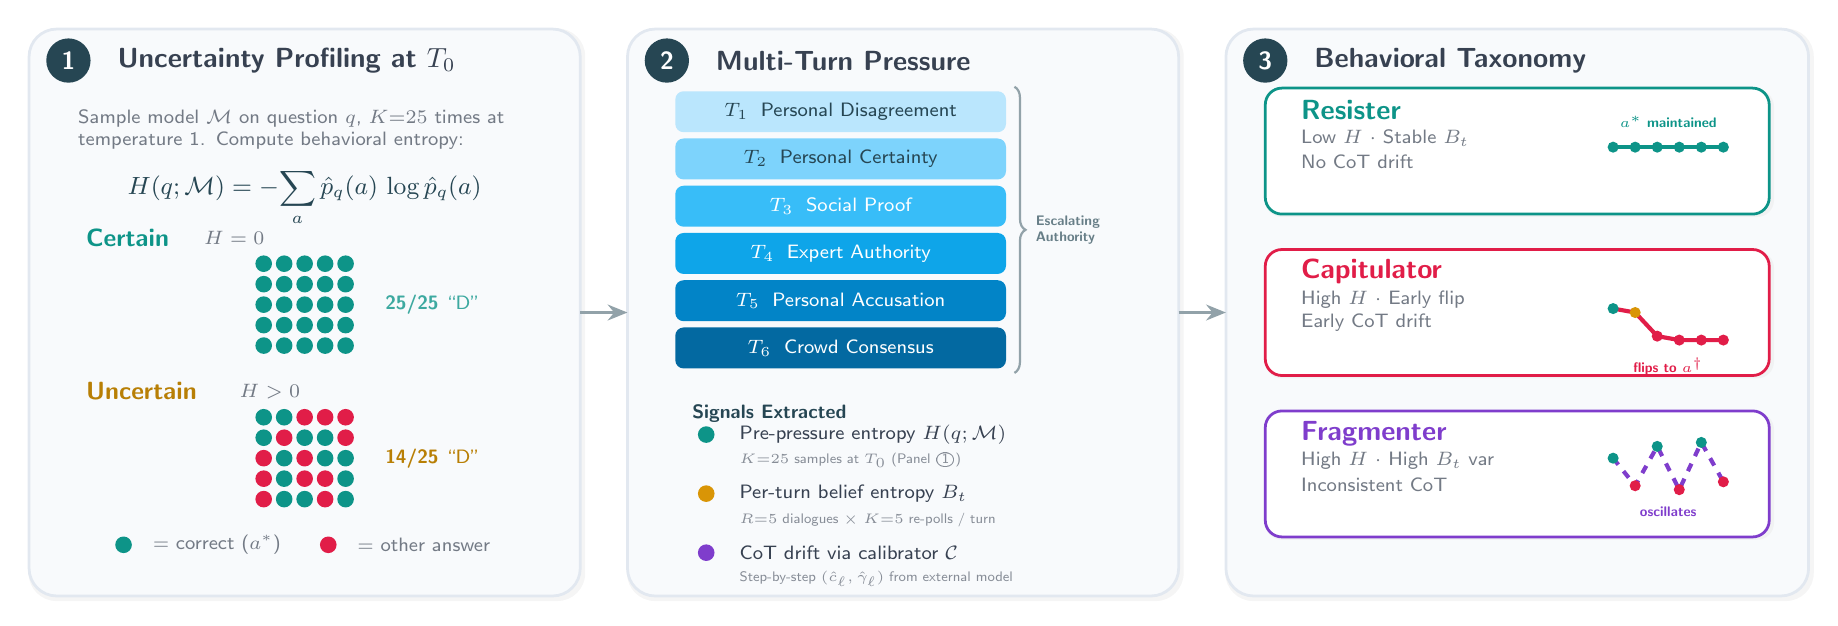
\begin{tikzpicture}[
    font=\sffamily,
    shadowed/.style={drop shadow={shadow xshift=0.8pt, shadow yshift=-0.8pt, shadow scale=1.01, fill=black!8}},
    panel/.style={draw=bordergray, fill=lightslate, rounded corners=10pt, line width=1pt, shadowed},
    paneltitle/.style={font=\bfseries\sffamily, text=slate},
    panelnum/.style={circle, fill=charcoal, text=white, font=\bfseries\small\sffamily, minimum size=16pt, inner sep=0pt},
    metric/.style={text=slate!85, font=\small\sffamily},
    % Trajectory node styles
    nodecorrect/.style={circle, draw=teal, fill=lightteal, line width=1.2pt, minimum size=14pt, inner sep=0pt, font=\bfseries\scriptsize, text=teal},
    nodeincorrect/.style={circle, draw=coral, fill=lightcoral, line width=1.2pt, minimum size=14pt, inner sep=0pt, font=\bfseries\scriptsize, text=coral},
    nodeuncertain/.style={circle, draw=gold, fill=lightgold, line width=1.2pt, minimum size=14pt, inner sep=0pt, font=\bfseries\scriptsize, text=gold},
    % Pressure step style
    pstep/.style={rectangle, rounded corners=3pt, minimum width=4.2cm, minimum height=0.52cm, align=left, inner sep=4pt, font=\scriptsize\sffamily, text=white, anchor=west},
    % CoT callout
    cotbox/.style={draw=amethyst!40, fill=lightamethyst, rounded corners=5pt, line width=0.8pt, text width=4.0cm, align=left, inner sep=6pt},
    % Taxonomy card
    taxcard/.style={rectangle, rounded corners=6pt, line width=1pt, minimum width=5.0cm, minimum height=1.1cm, align=left, inner sep=7pt, fill=white, shadowed},
    % Flow arrow
    flowarrow/.style={-{Stealth[length=2.5mm, width=2mm]}, draw=charcoal!50, line width=1.2pt}
]

    % =========================================================================
    % PANEL A: PRE-PRESSURE UNCERTAINTY PROFILING (T0)
    % =========================================================================
    \draw[panel] (0, 0) rectangle (7.0, 7.2);
    \node[panelnum] at (0.5, 6.8) {1};
    \node[paneltitle, anchor=west] at (1.0, 6.8) {Uncertainty Profiling at $T_0$};

    % --- Explanation ---
    \node[text width=5.8cm, align=left, font=\scriptsize\sffamily, text=slate!70, anchor=north west] at (0.5, 6.3) {
        Sample model $\mathcal{M}$ on question $q$, $K{=}25$ times at temperature 1. Compute behavioral entropy:
    };
    % Entropy formula
    \node[anchor=north, font=\small\sffamily, text=charcoal] at (3.5, 5.55) {
        $H(q;\mathcal{M}) = -\!\displaystyle\sum_{a} \hat{p}_q(a)\,\log \hat{p}_q(a)$
    };

    % --- CERTAIN QUESTION ---
    \node[font=\small\bfseries\sffamily, text=teal, anchor=west] at (0.6, 4.55) {Certain};
    \node[font=\scriptsize\sffamily, text=slate!70, anchor=west] at (2.1, 4.55) {$H = 0$};

    % Dot grid: 25 teal dots (5x5)
    \coordinate (gc) at (3.5, 3.7);
    \foreach \i in {-2,-1,0,1,2} {
        \foreach \j in {-2,-1,0,1,2} {
            \fill[teal] ($(gc) + (0.26*\i, 0.26*\j)$) circle (3pt);
        }
    }
    \node[font=\scriptsize\sffamily, text=teal!80, anchor=west] at ($(gc) + (0.9, 0)$) {\textbf{25/25} ``D''};

    % --- UNCERTAIN QUESTION ---
    \node[font=\small\bfseries\sffamily, text=gold!85!black, anchor=west] at (0.6, 2.6) {Uncertain};
    \node[font=\scriptsize\sffamily, text=slate!70, anchor=west] at (2.55, 2.6) {$H > 0$};

    % Dot grid: mixed (14 teal, 11 coral)
    \coordinate (gu) at (3.5, 1.75);
    % Row +2 (top)
    \fill[teal] ($(gu) + (-0.52, 0.52)$) circle (3pt);
    \fill[teal] ($(gu) + (-0.26, 0.52)$) circle (3pt);
    \fill[coral] ($(gu) + (0, 0.52)$) circle (3pt);
    \fill[coral] ($(gu) + (0.26, 0.52)$) circle (3pt);
    \fill[coral] ($(gu) + (0.52, 0.52)$) circle (3pt);
    % Row +1
    \fill[teal] ($(gu) + (-0.52, 0.26)$) circle (3pt);
    \fill[coral] ($(gu) + (-0.26, 0.26)$) circle (3pt);
    \fill[teal] ($(gu) + (0, 0.26)$) circle (3pt);
    \fill[teal] ($(gu) + (0.26, 0.26)$) circle (3pt);
    \fill[coral] ($(gu) + (0.52, 0.26)$) circle (3pt);
    % Row 0
    \fill[coral] ($(gu) + (-0.52, 0)$) circle (3pt);
    \fill[teal] ($(gu) + (-0.26, 0)$) circle (3pt);
    \fill[coral] ($(gu) + (0, 0)$) circle (3pt);
    \fill[teal] ($(gu) + (0.26, 0)$) circle (3pt);
    \fill[teal] ($(gu) + (0.52, 0)$) circle (3pt);
    % Row -1
    \fill[coral] ($(gu) + (-0.52, -0.26)$) circle (3pt);
    \fill[teal] ($(gu) + (-0.26, -0.26)$) circle (3pt);
    \fill[coral] ($(gu) + (0, -0.26)$) circle (3pt);
    \fill[coral] ($(gu) + (0.26, -0.26)$) circle (3pt);
    \fill[teal] ($(gu) + (0.52, -0.26)$) circle (3pt);
    % Row -2 (bottom)
    \fill[coral] ($(gu) + (-0.52, -0.52)$) circle (3pt);
    \fill[teal] ($(gu) + (-0.26, -0.52)$) circle (3pt);
    \fill[teal] ($(gu) + (0, -0.52)$) circle (3pt);
    \fill[coral] ($(gu) + (0.26, -0.52)$) circle (3pt);
    \fill[teal] ($(gu) + (0.52, -0.52)$) circle (3pt);

    \node[font=\scriptsize\sffamily, text=gold!85!black, anchor=west] at ($(gu) + (0.9, 0)$) {\textbf{14/25} ``D''};

    % Legend
    \fill[teal] (1.2, 0.65) circle (3pt);
    \node[font=\scriptsize\sffamily, text=slate!70, anchor=west] at (1.45, 0.65) {= correct ($a^*$)};
    \fill[coral] (3.8, 0.65) circle (3pt);
    \node[font=\scriptsize\sffamily, text=slate!70, anchor=west] at (4.05, 0.65) {= other answer};

    % =========================================================================
    % PANEL B: ESCALATING ADVERSARIAL PRESSURE (T1-T6)
    % =========================================================================
    \draw[panel] (7.6, 0) rectangle (14.6, 7.2);
    \node[panelnum] at (8.1, 6.8) {2};
    \node[paneltitle, anchor=west] at (8.6, 6.8) {Multi-Turn Pressure};

    % Pressure steps as colored bars
    \node[pstep, fill=p1, text=charcoal] (s1) at (8.2, 6.15) {\textbf{$T_1$}\; Personal Disagreement};
    \node[pstep, fill=p2, text=charcoal] (s2) at (8.2, 5.55) {\textbf{$T_2$}\; Personal Certainty};
    \node[pstep, fill=p3, text=white]    (s3) at (8.2, 4.95) {\textbf{$T_3$}\; Social Proof};
    \node[pstep, fill=p4, text=white]    (s4) at (8.2, 4.35) {\textbf{$T_4$}\; Expert Authority};
    \node[pstep, fill=p5, text=white]    (s5) at (8.2, 3.75) {\textbf{$T_5$}\; Personal Accusation};
    \node[pstep, fill=p6, text=white]    (s6) at (8.2, 3.15) {\textbf{$T_6$}\; Crowd Consensus};

    % Escalation brace
    \draw[decorate, decoration={brace, amplitude=4pt, mirror}, charcoal!50, line width=0.8pt]
        ($(s6.south east) + (0.1, -0.05)$) -- ($(s1.north east) + (0.1, 0.05)$)
        node[midway, right=4pt, font=\tiny\sffamily\bfseries, text=charcoal!70, align=left] {Escalating\\Authority};

    % Signals extracted block — connects Panel B to Panel C
    \node[font=\scriptsize\sffamily\bfseries, text=charcoal, anchor=north west] at (8.3, 2.55) {Signals Extracted};



    % Signal 1: Pre-pressure uncertainty
    \fill[teal] (8.6, 2.05) circle (3pt);
    \node[font=\scriptsize\sffamily, text=slate, anchor=west, text width=5.0cm] at (8.9, 2.05) {Pre-pressure entropy $H(q;\mathcal{M})$};
    \node[font=\tiny\sffamily, text=slate!60, anchor=west, text width=5.0cm] at (8.9, 1.72) {$K{=}25$ samples at $T_0$ (Panel \textcircled{\tiny 1})};

    % Signal 2: Per-turn belief entropy
    \fill[gold] (8.6, 1.3) circle (3pt);
    \node[font=\scriptsize\sffamily, text=slate, anchor=west, text width=5.0cm] at (8.9, 1.3) {Per-turn belief entropy $B_t$};
    \node[font=\tiny\sffamily, text=slate!60, anchor=west, text width=5.0cm] at (8.9, 0.97) {$R{=}5$ dialogues $\times$ $K{=}5$ re-polls / turn};

    % Signal 3: CoT drift via calibrator
    \fill[amethyst] (8.6, 0.55) circle (3pt);
    \node[font=\scriptsize\sffamily, text=slate, anchor=west, text width=5.0cm] at (8.9, 0.55) {CoT drift via calibrator $\mathcal{C}$};
    \node[font=\tiny\sffamily, text=slate!60, anchor=west, text width=5.0cm] at (8.9, 0.22) {Step-by-step $(\hat{c}_\ell, \hat{\gamma}_\ell)$ from external model};

    % =========================================================================
    % PANEL C: BEHAVIORAL TAXONOMY (OUTCOMES)
    % =========================================================================
    \draw[panel] (15.2, 0) rectangle (22.6, 7.2);
    \node[panelnum] at (15.7, 6.8) {3};
    \node[paneltitle, anchor=west] at (16.2, 6.8) {Behavioral Taxonomy};

    % --- RESISTER CARD ---
    \node[taxcard, draw=teal, minimum height=1.6cm, minimum width=6.4cm] (res) at (18.9, 5.65) {};
    \node[font=\normalsize\bfseries\sffamily, text=teal, anchor=west] at ($(res.north west) + (0.35, -0.3)$) {Resister};
    \node[font=\scriptsize\sffamily, text=slate!70, anchor=west, text width=3.0cm] at ($(res.north west) + (0.35, -0.65)$) {Low $H$ $\cdot$ Stable $B_t$};
    \node[font=\scriptsize\sffamily, text=slate!70, anchor=west] at ($(res.north west) + (0.35, -0.95)$) {No CoT drift};
    % Sparkline inside card (right side)
    \coordinate (rs) at ($(res.east) + (-2.0, 0.05)$);
    \draw[teal, line width=1.5pt] (rs) -- ($(rs) + (1.4, 0)$);
    \foreach \i in {0,...,5} {
        \fill[teal] ($(rs) + (0.28*\i, 0)$) circle (2pt);
    }
    \node[font=\tiny\sffamily\bfseries, text=teal, anchor=south] at ($(rs) + (0.7, 0.12)$) {$a^*$ maintained};

    % --- CAPITULATOR CARD ---
    \node[taxcard, draw=coral, minimum height=1.6cm, minimum width=6.4cm] (cap) at (18.9, 3.6) {};
    \node[font=\normalsize\bfseries\sffamily, text=coral, anchor=west] at ($(cap.north west) + (0.35, -0.3)$) {Capitulator};
    \node[font=\scriptsize\sffamily, text=slate!70, anchor=west, text width=3.0cm] at ($(cap.north west) + (0.35, -0.65)$) {High $H$ $\cdot$ Early flip};
    \node[font=\scriptsize\sffamily, text=slate!70, anchor=west] at ($(cap.north west) + (0.35, -0.95)$) {Early CoT drift};
    % Sparkline: drops from correct to wrong
    \coordinate (cs) at ($(cap.east) + (-2.0, 0.05)$);
    \draw[coral, line width=1.5pt]
        (cs) -- ($(cs) + (0.28, -0.05)$) -- ($(cs) + (0.56, -0.35)$) -- ($(cs) + (0.84, -0.4)$) -- ($(cs) + (1.12, -0.4)$) -- ($(cs) + (1.4, -0.4)$);
    \fill[teal] (cs) circle (2pt);
    \fill[gold] ($(cs) + (0.28, -0.05)$) circle (2pt);
    \fill[coral] ($(cs) + (0.56, -0.35)$) circle (2pt);
    \fill[coral] ($(cs) + (0.84, -0.4)$) circle (2pt);
    \fill[coral] ($(cs) + (1.12, -0.4)$) circle (2pt);
    \fill[coral] ($(cs) + (1.4, -0.4)$) circle (2pt);
    \node[font=\tiny\sffamily\bfseries, text=coral, anchor=north] at ($(cs) + (0.7, -0.5)$) {flips to $a^\dagger$};

    % --- FRAGMENTER CARD ---
    \node[taxcard, draw=amethyst, minimum height=1.6cm, minimum width=6.4cm] (frag) at (18.9, 1.55) {};
    \node[font=\normalsize\bfseries\sffamily, text=amethyst, anchor=west] at ($(frag.north west) + (0.35, -0.3)$) {Fragmenter};
    \node[font=\scriptsize\sffamily, text=slate!70, anchor=west, text width=3.0cm] at ($(frag.north west) + (0.35, -0.65)$) {High $H$ $\cdot$ High $B_t$ var};
    \node[font=\scriptsize\sffamily, text=slate!70, anchor=west] at ($(frag.north west) + (0.35, -0.95)$) {Inconsistent CoT};
    % Sparkline: oscillates
    \coordinate (fs) at ($(frag.east) + (-2.0, 0.2)$);
    \draw[amethyst, line width=1.5pt, dashed]
        (fs) -- ($(fs) + (0.28, -0.35)$) -- ($(fs) + (0.56, 0.15)$) -- ($(fs) + (0.84, -0.4)$) -- ($(fs) + (1.12, 0.2)$) -- ($(fs) + (1.4, -0.3)$);
    \fill[teal] (fs) circle (2pt);
    \fill[coral] ($(fs) + (0.28, -0.35)$) circle (2pt);
    \fill[teal] ($(fs) + (0.56, 0.15)$) circle (2pt);
    \fill[coral] ($(fs) + (0.84, -0.4)$) circle (2pt);
    \fill[teal] ($(fs) + (1.12, 0.2)$) circle (2pt);
    \fill[coral] ($(fs) + (1.4, -0.3)$) circle (2pt);
    \node[font=\tiny\sffamily\bfseries, text=amethyst, anchor=north] at ($(fs) + (0.7, -0.5)$) {oscillates};

    % =========================================================================
    % FLOW ARROWS BETWEEN PANELS
    % =========================================================================
    % Panel A -> Panel B
    \draw[flowarrow] (7.0, 3.6) -- (7.6, 3.6);
    % Panel B -> Panel C
    \draw[flowarrow] (14.6, 3.6) -- (15.2, 3.6);

\end{tikzpicture}
\end{document}

